\documentclass[10pt,letterpaper]{article}
%\usepackage[landscape]{geometry}
\usepackage{amsfonts}
\usepackage{graphicx}
\usepackage{bbm}
\title{Time Delay for a Filtered Ramp Signal}
\author{Matt Roelle}
\begin{document}
\maketitle
Time delay associated with a filter may be used to feed-forward a signal based on its derivative, a simplistic estimator. For example, a spinning motor position can be filtered for accuracy. If speed is constant, the current position can be calculated from a filtered position, the velocity, and the time-delay associated with the filter.

Classes of finite-impulse-response filters have fixed time delay for any input. It might be initially surprising that an IIR can also have constant delay. Any shock may evaporate when the constant delay is isolated to only specific input signals. In fact, there are two degenerate signals which have predictable delays for unity-gain transfer functions. First, and most obviously, a constant signal has constant zero time delay. Second, and pertinant to a spinning motor, a ramp signal has constant time delay. This constant delay may be calculated directly from filter transfer function coefficiencts. The soution is provided here and derived in later sections.

For unity-gain discrete transfer functions of the form $H(z)=\frac{B(z)}{A(z)}$, the time delay $t_d$ is
\begin{eqnarray}
t_d = T_s\frac{\mathbb{N}^T(B-A)}{\mathbbm{1}^TA}
\label{eqn:td_discrete_vectors}
\end{eqnarray}
where $A$ and $B$ are vectors of transfer function coefficients ($A$ is zero-padded as necessary), $\mathbbm{1}$ is a vector of ones, and $\mathbb{N}$ is a vector of natural numbers starting from zero. Equation~\ref{eqn:td_discrete_vectors} is the vector form of derivation via summations, equation~\ref{eqn:td_discrete_summations}.

For unity-gain continuous transfer functions of the form $H(s)=\frac{B(s)}{A(s)}$, where $B(s) = b_0s^n + b_1s^{n-1}\cdots + b_{n-1}s + b_n$ and $A(s) = a_0s^m + a_1s^{m-1}\cdots + a_{m-1}s + a_m$, the time delay $t_d$ is
\begin{eqnarray}
t_d = \frac{b_{n-1} - a_{m-1}}{a_m}
\label{eqn:td_continuous_vectors}
\end{eqnarray}

Note: If a ramp signal (e.g. motor position) is encoded in quadrature sine and cosine signals (e.g. a common absolute rotational position sensor) filtered with a unity-gain transfer function, the time delay on the decoded ramp is (\textit{seems to be}) given by equations \ref{eqn:td_discrete_vectors} and \ref{eqn:td_continuous_vectors} despite intuition for higher (or not-constant) delay on the quadrature signals.

\section*{Discrete Filter Derivation}
First, consider the general form of a filter in the form of the shift operator
\begin{eqnarray}
\frac{B(q)}{A(q)}=\frac{b_0q^n + b_1q^{n-1}\cdots + b_{n-1}q + b_n}
                       {q^m + a_1q^{m-1}\cdots + a_{m-1}q + a_m}
\end{eqnarray}
or in terms of time-steps
\begin{eqnarray}
y(k) + a_1y(k-1) + \cdots && \nonumber \\
+ a_{m-1}y(k-m+1) + a_my(k-m) &=& \nonumber \\
b_0u(k-m+n) + b_1u(k-m+n-1)\cdots && \nonumber \\
+ b_{n-1}u(k-m+1) + b_nu(k-m) &&
\label{eqn:timestep}
\end{eqnarray}

If $u$ is a ramp, each previous point is a fixed distance before the last. For one step
\begin{eqnarray}
u(k-1) &=&  u(k) - \Delta
\end{eqnarray}
or for several
\begin{eqnarray}
u(k-n) &=&  u(k) - n\Delta
\end{eqnarray}

Similarly, $y$ is also a ramp and for a unity gain transfer function the distance travelled each time step is the same as the input.
\begin{eqnarray}
y(k-n) &=&  y(k) - n\Delta
\end{eqnarray}

The distance, $\Delta$ may be substituted in equation \ref{eqn:timestep} for prior time-steps
\begin{eqnarray}
y(k) + a_1\left(y(k) - \Delta\right) + \cdots && \nonumber\\ 
+ a_{m-1}\left(y(k) - (m-1)\Delta\right) +
a_m\left(y(k) - m\Delta\right) &=& \nonumber\\
b_0\left(u(k) - (m-n)\Delta\right) + 
b_1\left(u(k) - (m-n+1)\Delta\right) + \cdots && \nonumber\\
+ b_{n-1}\left(u(k) - (m-1)\Delta\right) + 
b_n\left(u(k) - m\Delta\right) &&
\end{eqnarray}
Grouping terms yields a few simple summations
\begin{eqnarray}
y(k)\sum_{i=0}^m a_i - \Delta\sum_{i=0}^m a_ii = u(k)\sum_{i=0}^n b_i - \Delta\sum_{i=0}^n b_i(i+m-n)
\end{eqnarray}
Since the filter is unity gain
\begin{eqnarray}
\sum_{i=0}^m a_i =  \sum_{i=0}^n b_i
\end{eqnarray}
This equality allows the grouping of the difference between the current filter input and output.
\begin{eqnarray}
u(k) - y(k) = \Delta\frac{\sum\limits_{i=0}^n b_i(i+m-n) - \sum\limits_{i=0}^m a_ii}{\sum\limits_{i=0}^m a_i}
\end{eqnarray}
The time delay, $t_d$, is the amount of lag divided by the velocity, $\dot{u}$.
\begin{eqnarray}
t_d = \frac{u(k) - y(k)}{\dot{u}}
\end{eqnarray}
The velocity for the ramp is just the distance divided by sample time, $T_s$.
\begin{eqnarray}
\dot{u} &=& \frac{\Delta}{T_s}\\
t_d &=& \frac{u(k) - y(k)}{\Delta}T_s
\end{eqnarray}

So, finally
\begin{eqnarray}
t_d = T_s\frac{\sum\limits_{i=0}^n b_i(i+m-n) - \sum\limits_{i=0}^m a_ii}{\sum\limits_{i=0}^m a_i}
\end{eqnarray}
and if $m=n$
\begin{eqnarray}
t_d = T_s\frac{\sum\limits_{i=0}^m i(b_i - a_i)}{\sum\limits_{i=0}^m a_i}
\label{eqn:td_discrete_summations}
\end{eqnarray}
This equation is shown with vectors instead of summations in equation~\ref{eqn:td_discrete_vectors}.

\section*{Continuous Filter Derivation}
First, consider the general form of a filter
\begin{eqnarray}
\frac{B(s)}{A(s)}=\frac{b_0s^n + b_1s^{n-1}\cdots + b_{n-1}s + b_n}
                       {s^m + a_1s^{m-1}\cdots + a_{m-1}s + a_m}
\end{eqnarray}

The time delay on a signal $u(t)$ filtered to $y(t)$ is the shift $u(t)-y(t)$ divided by the (constant) velocity, $\dot{u}$.
\begin{eqnarray}
\frac{u(t_\infty) - y(t_\infty)}{\dot{u}} &=& 
\frac{\left(1 - H(s)\right)u(t_\infty)}{su(t_\infty)}\\
t_d &=& \lim_{s\rightarrow0}\frac{A(s) - B(s)}{A(s)s}
\end{eqnarray}
 
For the transfer function to have unity gain, from the final-value theorem we know
\begin{eqnarray}
a_m=b_n
\end{eqnarray}
Thus, the constant term of $A(s)-B(s)$ cancels allowing the extra $s$ in the denominator to cancel in the numerator.
\begin{eqnarray}
t_d = \lim_{s\rightarrow0}
\frac{\left(s^m + a_1s^{m-1}\cdots + a_{m-1}s\right) - \left(b_0s^n + b_1s^{n-1}\cdots + b_{n-1}s\right)}
{\left(s^m + a_1s^{m-1}\cdots + a_{m-1}s + a_m\right)s}\\
t_d = \lim_{s\rightarrow0}
\frac{\left(s^{m-1} + a_1s^{m-2}\cdots + a_{m-1}\right) - \left(b_0s^{n-1} + b_1s^{n-2}\cdots + b_{n-1}\right)}
{s^m + a_1s^{m-1}\cdots + a_{m-1}s + a_m}
\end{eqnarray}
Which can be solved with simple substituion of zero for $s$ resulting in equation~\ref{eqn:td_continuous_vectors}.

\begin{figure}
\centering
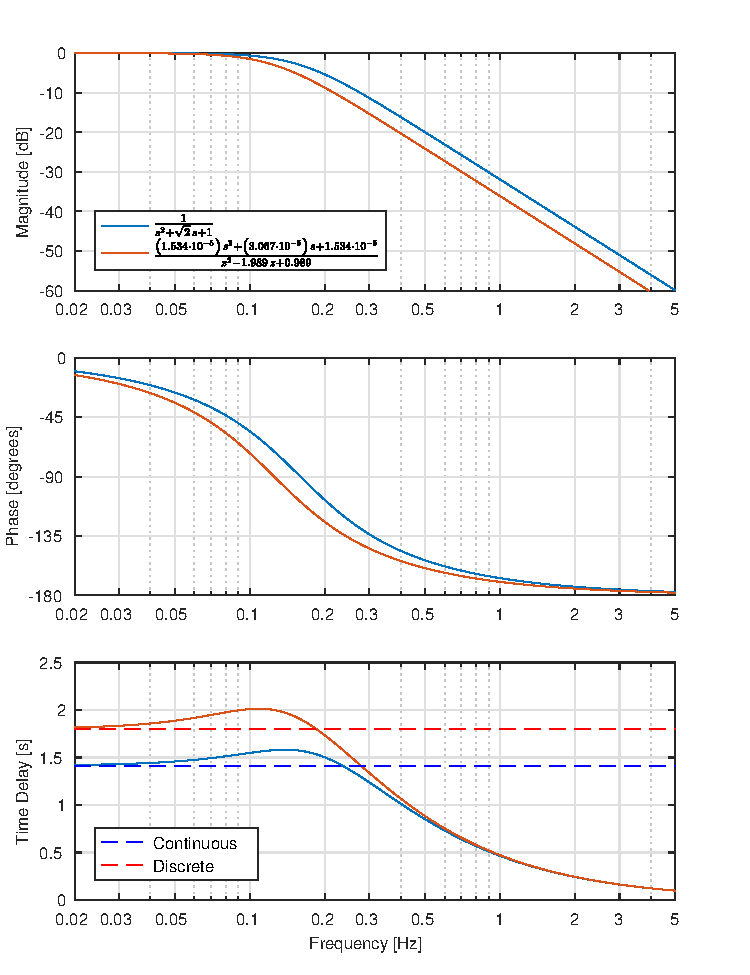
\includegraphics{RampIIRDelay2.pdf}
\caption{The Bode plot of a specific discrete filter shows the DC delay approaching the fixed ramp delay.}
\label{fig:Bode}
\end{figure}


\newpage
\subsection*{Matlab code}
\begin{verbatim}
Ts = 2e-4;
[B, A] = butter(6, 0.02);
td = Ts*(B - A)*(0:length(A)-1)'/sum(A);

t = (0:Ts:2);
v = 7;
x = t*v;

tfilt = filter(B, A, t);
xfilt = filter(B, A, x);

rng = (5e3:9e3);
fprintf('Time delay, numerical:  %0.2f ms\n', ...
        (mean(x(rng) - xfilt(rng))/v)*1e3);
fprintf('Time delay, analytical: %0.2f ms\n', td*1e3);

fprintf('Position shift, numerical:  %0.2f mm\n', ...
        (mean(x(rng) - xfilt(rng)))*1e3);
fprintf('Position shift, analytical: %0.2f mm\n', v*td*1e3);
\end{verbatim}
\subsection*{Output, 7 m/s}
\begin{verbatim}
>>
Time delay, numerical:  12.29 ms
Time delay, analytical: 12.29 ms
Position shift, numerical:  86.06 mm
Position shift, analytical: 86.06 mm
\end{verbatim}
\end{document}

